%
% File:     chapter-schedule.tex
% Author:   awl8049
% Revision: $Revision: 2.1 $
%
\chapter{A Thermal Aware Scheduler}
\label{chp:schedule}
The scheduler in an operating system is responsible for making two
decisions in each time quantum: (1) thread scheduling, i.e., deciding
the next thread to run on an available core and (2) load balancing,
namely, distributing workload evenly across all cores, with existing
implementations mostly focusing on performance.  Our TAS (Thermal Aware
Scheduler) incorporates a heuristic scheduling algorithm in a popular
scheduler (i.e., ULE in the FreeBSD operating system) for thermal stress
reduction on a multi-core processor while meeting the Single Process,
Multiple Data requirements
of equal execution progress and maximum parallelism exploitation.

\begin{figure}[t] \centering
  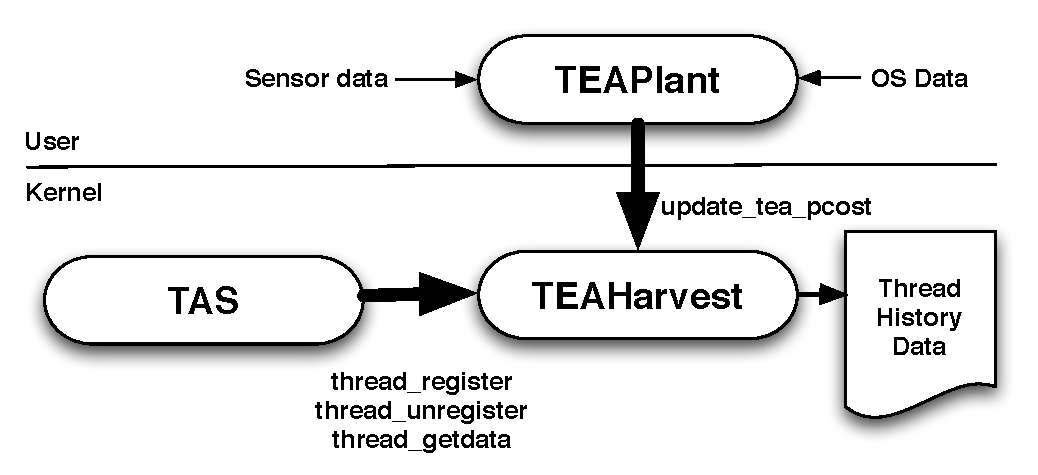
\includegraphics[scale=0.45]{tasdesign}
  \caption{TEAPlant and TEAHarvest data collection.}
  \label{fig:teaplant}
\end{figure}

\section{Thermal Predictors}
\label{sec:therm-pred-design} 
We enhance the existing FreeBSD operating system to maintain information
required by the thermal estimator. Our design is based on the concept of
Task Activity Vectors (TAVs) introduced earlier \cite{Merkel2008a}, with
a vector for each kernel thread to store the required history in order
to make sound prediction.  Generally, the more additional space is
employed for history maintenance, the higher benefit our thermal
scheduling gains.

The high-level system design of TAS is shown in
\figurename~\ref{fig:teaplant}.  A user-level daemon process collects
required information to compute the time-series predictions for $\Theta$
and $C_{\theta}$. Similar to the energy CAPs described in
Section~\ref{sec:chaospredict}, tCAPs use $n=5$ future observations and
$p=100$ past observations to compute predictions. Temperature readings
are collected by this process from the digital temperature sensor
associated with a core.  Similarly, processor performance counters are
gathered by the same process, with both sets of metrics used to generate
estimates. Estimates are posted via a system call interface to a device
driver that collects the data for use by the currently executing thread.
The scheduler queries this driver via a kernel function call interface
when making scheduling decisions to determine the $\Theta$ and
$C_{\theta}$ estimates associated with a thread.

\begin{figure}[t]
  \centering
  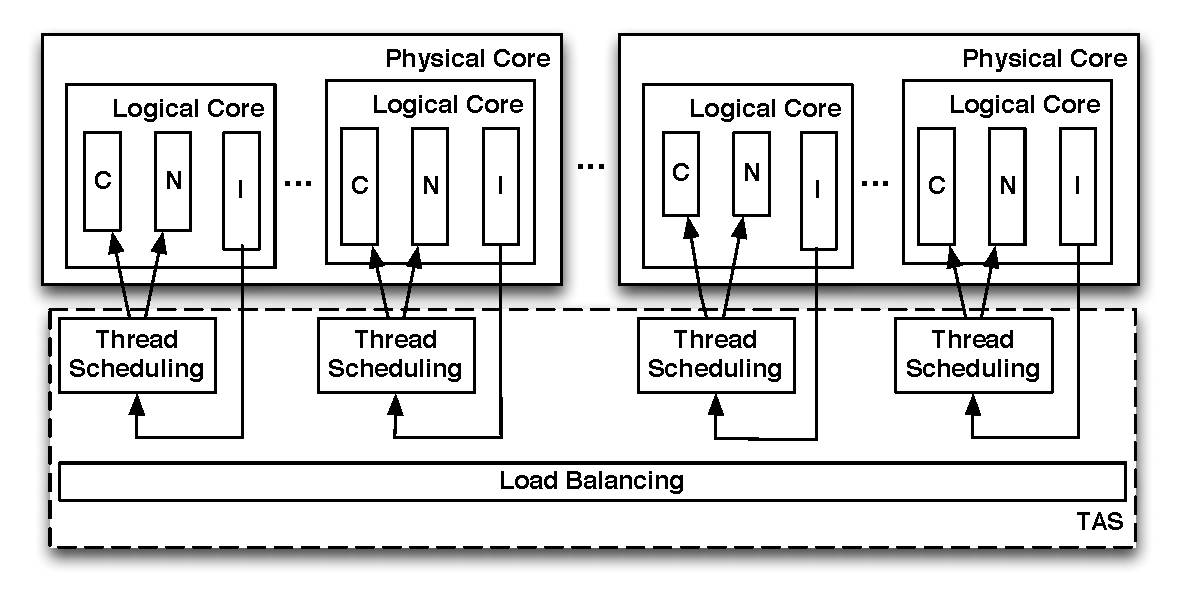
\includegraphics[width=1.0\linewidth,height=2.5in]{architecture}
  \caption{Internal structure of the TAS scheduler.}
  \label{fig:tasque}
\end{figure}
\section{Thread Scheduling}
\label{sec:selection} 
The scheduler uses the cost predictor for $C_{\theta}$ to predict a
thread's impact on core temperature and adjust the thread priority as
required to prevent an increase in core temperature. Each core will have
one process in a running state on each scheduling interval. All other
threads will assigned by TAS to one of three queue structures maintained
per logical core: an idle queue, a current queue, and the next queue
(illustrated in \figurename~\ref{fig:tasque}).  All idle threads are
added to the idle queue and threads from this queue are executed only when
the other two queues are empty.  The logical core executes all work on
the current queue in priority order and then swaps its current queue and
its next queue. For performance reasons, our implementation follows the
convention used by the existing FreeBSD ULE scheduler, placing real-time
and interrupt threads on the current queue.  This is reasonable,
given that real-time thread deadlines must be satisfied and
interrupt service routines are typically short in length.
Meanwhile, all other non-idle threads are assigned to either the current or next
queue based upon computing an interactivity score, $I$, for each thread, as follows:
\begin{equation}
\label{eq:interactsleeprun} 
I =   
\begin{cases}
  S / (SL/RUN) & \text{if sleep time} \geq \text{run time}\\
  (S/ (SL / RUN))+S & \text{if run time} < \text{sleep time}
\end{cases}
\end{equation}
where $S$ is the scaling factor of the
maximum interactivity score divided by two, and $SL$ and $RUN$ refer
respectively to the cumulative sleep and run times for the thread.
A thread with its $I$ score smaller than a predefined threshold means that
the thread had run for a very short duration during the last time window,
indicating an interactive nature of the thread (e.g., an interactive thread).   
Hence, threads whose scores fall below a predefined threshold are considered
interactive and are assigned to the current queue, with all other non-idle
threads assigned to the next queue.

\begin{figure}[t]
  \centering
  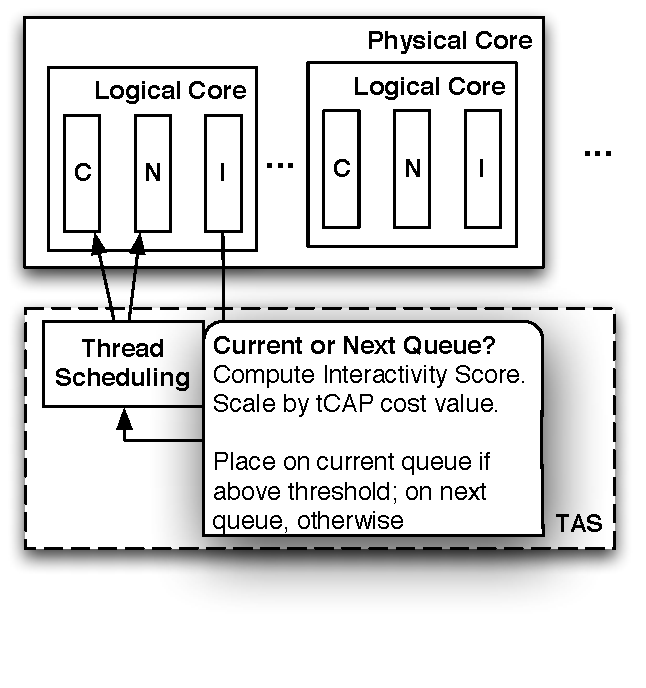
\includegraphics[width=1.0\linewidth,height=4in]{threadselect}
  \caption{TAS thermal queue selection.}
  \label{fig:tasselect}
\end{figure}

For our TAS, the interactivity score $I$ is scaled by the predicted
value of $C_{\theta}$, normalized to a percentage value.  It was shown
previously \cite{Zhou2010b} that the greatest thermal benefit occurred
when a scheduler favored the thread which moved the core temperature as
close as possible to the DTM threshold without actually triggering a DTM
event.  TAS achieves a similar effect by scaling the interactivity of a
thread by its normalized execution cost, thereby giving less ``thermally
costly'' threads greater opportunities for execution so as to moderate
the processor temperature.  Penalizing more thermally costly threads
reduces the opportunities for such threads to gain access to logical
cores, presenting similar advantages of techniques which artificially
inject slack into thread scheduling but without extra scheduling
overhead incurred to those techniques.  As shown in
\figurename~\ref{fig:tasselect}, threads with higher ``thermal cost''
will be scheduled onto the next queue and avoid contributing to the
thermal load of the processor.  Threads on the next queue will be
scheduled to run when the queues are switched and are guaranteed to run
at least once every two queue switches, which maintains fair sharing of
the processor.

\begin{figure}[t]
  \centering
  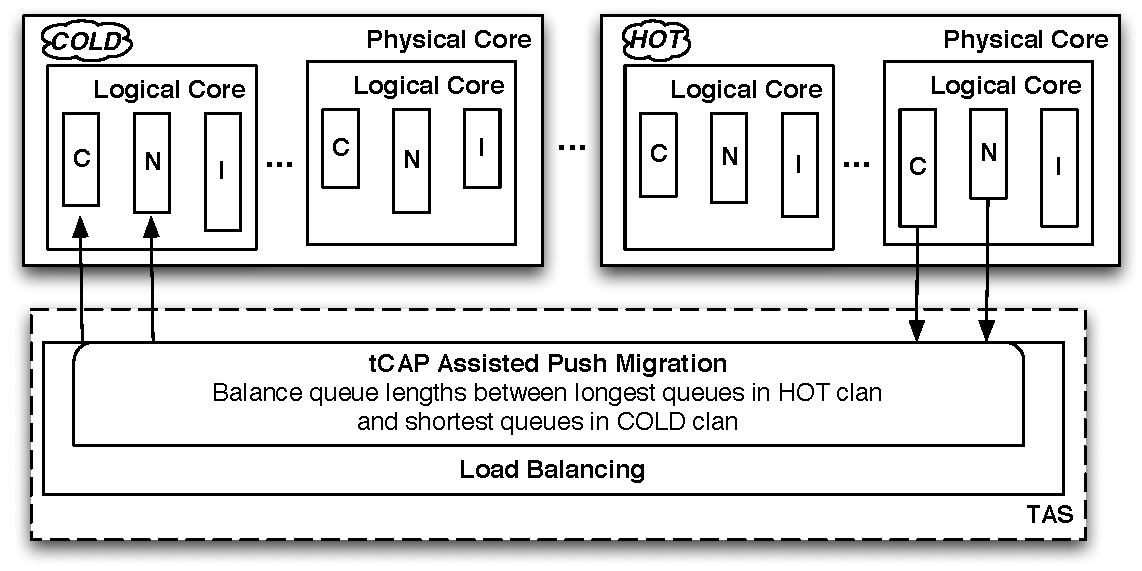
\includegraphics[width=1.0\linewidth,height=2.5in]{thbalance}
  \caption{TAS thermal load balancing.}
  \label{fig:tasbalance}
\end{figure}

\section{Load Balancing}
\label{sec:loadbalance} 
Load balancing distributes workload evenly across the available logical
cores, with the current implementation in the ULE scheduler mostly
aiming to maximize performance.  This work applies load balancing to
minimize thermal stress while seeking best performance.  As shown in
\figurename~\ref{fig:tasbalance}, TAS extends push migration by
organizing system cores into ``thermal clans'' based upon the
temperature and execution frequency.  Specifically, a local core is
assigned to one of the three thermal clans: Hot, Warm, and Cold, if its
on-die temperature is respectively 90\% or higher, between 75\% and
90\%, and below 75\% of the DTM threshold temperature.  Note that if a
physical core supports $\alpha$ threads, $\alpha$ logical cores will
result from the physical core, with their temperatures all equal to that
of the physical core.  In addition, logical cores are grouped into fast
and slow clans according to the execution frequencies of their
underlying physical cores.  This two-level categorization allows TAS to
manage work load distribution better from the thermal and performance
prospectives, by migrating work away from hot units with negligible
execution performance degradation.

For performance reasons, information about thermal clans of all logical
cores is maintained by the TEAHarvest thermal predictor driver.  The
driver allocates threads to local cores for execution, according to
thermal efficiency and cost estimates.  TAS scheduler queries the driver
to determine whether a core will move towards the DTM threshold
temperature if a thread becomes ready to execute on one of its logical
core.  In this way, TAS predicts whether a thread moves its assigned
core closer to a DTM event and adjusts the core's run-queue accordingly
to prevent DTM occurrence.

{\setlength{\abovecaptionskip}{0ex}
\begin{figure}[t] 
\centering
\begin{verbatim} 
                 BEGIN 
                   Determine if the logical core 
                     is in the Hot, Warm, or Cold clan.  
                   For each thread in the run queue 
                     BEGIN 
                       Use tCAP to estimate resulting 
                         temperature change if the thread 
                         is executed. 
                     END 
                   Determine least loaded core in the
                       Cold clan.  
                   Migrate the thread with worst impact 
                       on temperature to logical core in
                       the Cold clan most suitable from
                       the speed standpoint.  
                 END
\end{verbatim}
\caption{Pseudo code of TAS balancing algorithm.}
\label{fig:tascode}
\end{figure}
} 
On a periodic basis (i.e., once in every 500 ms), the TAS scheduler
executes the algorithm listed in \figurename~\ref{fig:tascode} to
balance the workload among logical cores, giving sufficient time for
overtaxed resources to thermally recover.  For each thread in the run
queue, TAS uses the tCAP to estimate the value of $\Theta$ for each
thread in the queue and predict the resulting change in temperature if
this thread were to execute.  It then moves the thread with the greatest
temperature impact to the least loaded logical core in the ``Cold''
clan, as illustrated in \figurename~\ref{fig:tasbalance}.  This way
results in workloads being moved away from thermally stressed logical
cores, while maintaining execution performance.

Execution performance is maintained by taking note of the location of
this logical core in the processor group topology.  The scheduler
inventories the processor when it starts execution and creates a
processor group structure that records the location of each logical core
n the hierarchy of physical processor sockets and physical
core~\cite{McKusick2004b}.  The decision of where to migrate the thread
is made based upon which logical cores in the Cold clan are located in
the topology, with preference given to logical cores that are sharing
last-level caches on the same processor.  For the example in
\figurename~\ref{fig:tasbalance}, the TAS would look to choose a
processor from the Cold clan by selecting (1) a thread on a logical core
with whom it shares a last-level cache, (2) a core on the same
processor, and, finally (3) to a core on the other processor.  Thus, TAS
respects thread cache affinity and minimizes the performance impact of
migration of threads between logical cores.

Periodically, the system reads the temperatures of all logical cores
and, if required, also moves a logical cores to a different thermal
clan.  It should be noted that the time required for a logical core to
recover from a thermal event is significantly longer than the interval
used for thread scheduling~\cite{Choi2007}. This allows our TAS to use a
much larger interval (2 seconds) between scans (across core
temperatures) to determine if any logical core must be assigned to a new
thermal clan for better scheduling outcomes.

% Following comment block used by GNU-EMACS and AUCTEX packages
% Please do not remove.
%%% Local Variables: 
%%% mode: latex
%%% TeX-master: "dissertation.tex"
%%% TeX-PDF-mode: t
%%% TeX-source-correlate-mode: t
%%% End: 
